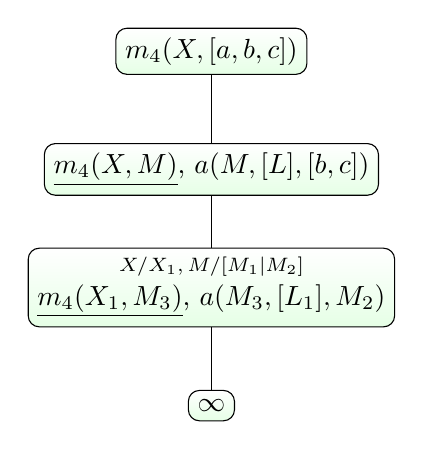
\begin{tikzpicture}[sibling distance=10em,
  every node/.style = {shape=rectangle, rounded corners,
    draw, align=center,
    top color=white, bottom color=green!10}]]
  \node {$m_4(X,[a,b,c])$}
    child { node {\underline{$m_4(X, M)$}, $a(M, [L], [b,c]$)}
      child { node {\scriptsize $X/X_1, M/[M_1|M_2]$\\\underline{$m_4(X_1, M_3)$}, $a(M_3, [L_1], M_2)$}
        child { node {$\infty$}}
      }
    };
\end{tikzpicture}